\chapter{Entwurf und Design}
\section{\acs{FPGA}-Design}
Nach der Festlegung der Anforderungen wurde mit der Konzeption und Entwurfsphase des gesamt Systemes sowie des \acs{FPGA}-Designs begonnen.

Hierbei wurde zuerst anhand der Anforderungen die Architektur des zu erstellenden FPGA-Designs festgelegt.

Die Kommunikation zwischen den einzelnen Modulen, besonders für den Datenaustausch, soll zum größten Teil mit einer \acs{AXI}-Stream basierten 
Schnittstelle umgesetzt werden. Für die, hauptsächlich zur Steuerung verwendete, Kommunikation zwischen \acs{FPGA}-Design und Rechenkern sollen
\acs{AXI}-Lite basierte Registerbänke verwendet werden.

In dem folgenden Entwurf nicht betrachtet werden die weiterhin notwendigen \acs{AXI}-Infrastruktur Blöcke welche, für die Kommunikation mit dem Rechenkern weiterhin noch benötigt werden,
jedoch nicht selbst umgesetzt werden. Eine Gesamtübersicht des Designs (mit \acs{AXI}-Infrastruktur) kann im Kapitel \ref{Chap:Impl} gefunden werden.

Es handelt sich um eine klassische \acs{QPSK}-Empfängerarchitektur mit direkter digitaler Abwärtsmischung.

\begin{figure}[h]
	\centering
	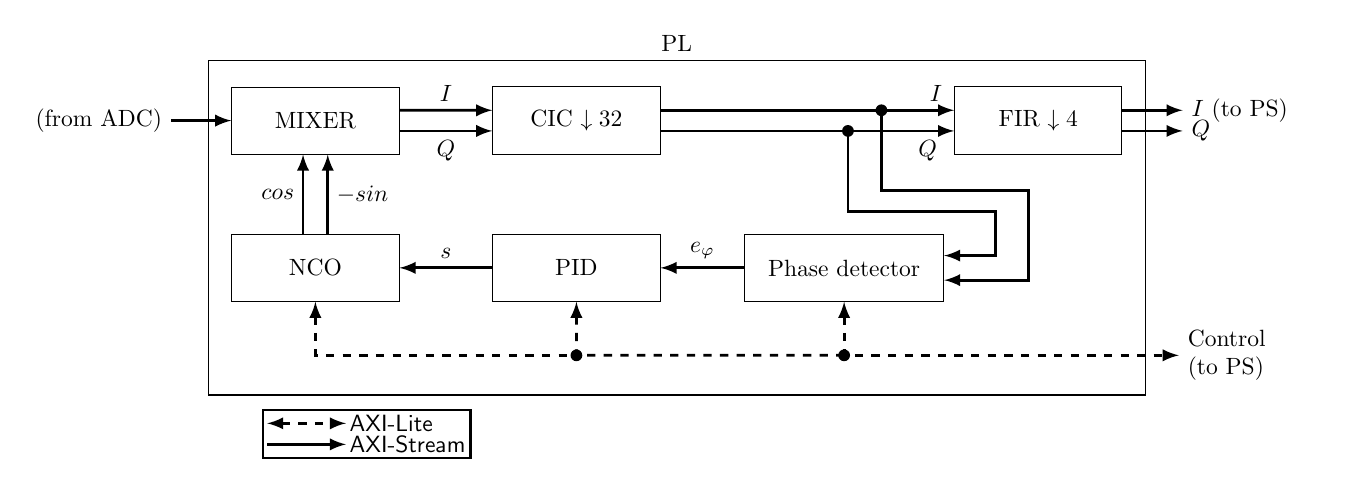
\begin{tikzpicture}[scale=0.85, every node/.style={scale=0.85}]
		\def\arow{7.0}
		\def\aarow{1.6}
		\def\abrow{5.5}
		\def\acrow{9.5}
		\def\adrow{12.4}
			
		\tikzset{
			basic/.style={rectangle,draw=black, top color=white,text centered},
			PLnode/.style={basic, inner sep=1em,minimum width=14cm, minimum height=5.0cm},	
			smallnode/.style={basic, inner sep=1em,minimum width=2.5cm, minimum height=1cm},
			branch/.style={fill,circle,minimum size=5pt,inner sep=0pt,outer sep=-1pt},
			sarrow/.style={->, >={latex}, line width=1.0pt},
    		carrow/.style={<->, >={latex}, dashed, line width=1.0pt}
 		}
 		
 		\node[PLnode, label=above:PL] (PL) at (\arow,1.5) {};

		% internal Nodes

 		\node[smallnode] (PL_NCO)   at (\aarow,0.9) {NCO};
	 	\node[smallnode] (PL_MIX) at (\aarow,3.1) {MIXER}; 		 
 		\node[smallnode] (PL_CIC) at (\abrow,3.1) {CIC $\downarrow 32$};
 		\node[smallnode] (PL_FIR) at (\adrow,3.1) {FIR $\downarrow 4$};
 		\node[smallnode] (PL_PID) at (\abrow,0.9) {PID};
 		\node[smallnode] (PL_PD) at  (\acrow,0.9) {Phase detector};

		% internal interconnect arrows

 		\draw[sarrow, ->] (PL_NCO.70) -- (PL_MIX.-70) node[midway,right] {$-sin$};
 		\draw[sarrow, ->] (PL_NCO.110) -- (PL_MIX.-110) node[midway,left] {$cos$};

 		\draw[sarrow, ->] (PL_MIX.7)  -- (PL_CIC.173) node[midway,above] {$I$};
 		\draw[sarrow, ->] (PL_MIX.-7) -- (PL_CIC.-173) node[midway,below] {$Q$};
	 	
	 	\draw[sarrow, ->] (PL_CIC.7)  -- ++(3.3,0) node[branch](bI){} -- (PL_FIR.173) node[near end, above] {$I$};
 		\draw[sarrow, ->] (PL_CIC.-7) -- ++(2.8,0) node[branch](bQ){} -- (PL_FIR.-173) node[near end, below] {$Q$};

 		\draw[sarrow, ->] (PL_PID.west)  -- (PL_NCO.east) node[midway,above] {$s$}; 		
 		\draw[sarrow, ->] (PL_PD.west)  -- (PL_PID.east) node[midway,above] {$e_\varphi$}; 		
 		
 		\draw[sarrow, ->] (bI)  |- ++(2.2, -1.2) |- (PL_PD.-7); 	
 		\draw[sarrow, ->] (bQ)  |- ++(2.2, -1.2) |- (PL_PD.7); 	

		% control connections
		
		\draw[carrow, <->] (PL_PD.south)  -- ++(0, -0.8) node[branch](bC0){} -- ++(5,0) node[right,text width=2cm]{Control\\(to PS)}; 
		\draw[carrow, <-] (PL_PID.south)  -- ++(0, -0.8) node[branch](bC1){} -- (bC0);
 		\draw[carrow, <-] (PL_NCO.south)  |- (bC1);
 		
 		% external connections
 		\draw[sarrow, ->] (PL_FIR.7)  -- ++(0.9,0) node[right] {$I$ (to PS)};
 		\draw[sarrow, ->] (PL_FIR.-7) -- ++(0.9,0) node[right] {$Q$};
 		\draw[sarrow, <-] (PL_MIX.west) -- ++(-0.9,0) node[left] {(from ADC)};
 		
 		% legend
 		\path ([xshift=35mm,yshift=-2mm]current bounding box.south west) node[matrix,anchor=north west,cells={nodes={font=\sffamily,anchor=west}}, draw,thick,inner sep=1pt]{
  			\draw[carrow](0,0) -- ++ (1,0); & \node{AXI-Lite};\\
  			\draw[sarrow](0,0) -- ++ (1,0); & \node{AXI-Stream};\\
 		};
	\end{tikzpicture}
	\caption{Architektur des \acs{FPGA}-Designs (ohne \acs{AXI}-Infrastruktur)}
\end{figure}

Die Hauptkomponenten des \acs{FPGA}-Designs werden in den folgenden Abschnitten noch etwas näher erklärt.

\subsection{Mischer (Mixer)}
Der Mischer hat die Aufgabe den von dem \acs{ADC} abgetasteten Datenstrom mit den, vom lokalen Oszillator erzeugten, Trägern zu multiplizieren und so das Nutzsignal in das
Basisband zu verschieben. Die besondere Schwierigkeit liegt hier dabei, dass der Mischer mit der Taktrate des \acs{ADC}s $f_{ADC}$ betrieben werden muss.

Für den Empfang von \acs{QPSK}-modulierten Daten ist es notwendig einen komplexen Mischer \textit{(sogenannter I/Q-Mischer)} zu verwenden.
Als Eingang dienen zwei vom lokalen Oszillator (\acs{NCO}) erzeugten Referenzsignale \textit{(Sinus/Kosinus)}, sowie der \acs{ADC}-Datenstrom ($x[n]$),
welche dann wie folgt Multipliziert werden: 
\begin{equation}
	I[n] = x[n]\cdot cos(2\pi\frac{f}{f_{ADC}}\cdot n) 
\end{equation}
\begin{equation}
	Q[n] = x[n]\cdot -sin(2\pi\frac{f}{f_{ADC}}\cdot n) 
\end{equation}

Es entsteht ein komplexer Datenstrom welcher dann für die weitere Verarbeitung genutzt werden kann:
\begin{equation}
	\underline{y}[n] = I[n] - j \cdot Q[n] = x[n]\cdot e^{j2\pi\frac{f}{f_{ADC}}\cdot n}
\end{equation}

Zusätzlich zu dem Signal im Basisband entsteht bei der Mischung immer auch eine Kopie des Signals bei dem doppelten der Trägerfrequenz.\cite{WPI_COSTAS}
Die nicht erwünschte Kopie wird anschließend durch die Verwendung eines Tiefpassfilters eliminiert. Diese Aufgabe übernimmt hier der \acs{CIC}-Dezimierungsfilter.

Ein- und Ausgabeschnittstellen des Mischers sollen als \acs{AXI}-Stream realisiert werden, wobei es notwendig ist jeden Taktzyklus einen neuen Datenwert
im Mischer zu verarbeiten. 

\subsection{Lokaler Oszillator (\acs{NCO})}
Der lokale Oszillator hat die Aufgabe die von dem Mischer verwendeten Referenzsignale zu erzeugen. 

Umgesetzt ist der lokale Oszillator als Numerisch gesteuerter Oszillator (\acs{NCO}). 
Die notwendige Sinus-/Kosinusignale werden hierbei durch die sogenannte direkte digitale Synthese (\acs{DDS}) erzeugt.

Dabei handelt es sich effektiv um einen Zähler (Phasen-Akkumulator, $n$-Bit breit) von welchem anschließend die untersten $m$-Bit verwendet werden
um die Ausgangsdatenwerte in einer Lookup-Tabelle nachzuschlagen.
Anhand der Schrittweite $s$ um welche der Phasen-Akkumulator jeden Taktzyklus erhöht wird lässt sich die Grundfrequenz der ausgegebenen Sinusschwingungen einstellen.

\begin{figure}[h]
	\centering
	\begin{tikzpicture}[scale=0.85, every node/.style={scale=0.85}]
		\def\arow{0.0}
		\def\brow{4.0}
		\def\crow{10.0}
			
		\tikzset{
			basic/.style={rectangle,draw=black, top color=white,text centered},
			smallnode/.style={basic, inner sep=1em,minimum width=2.5cm, minimum height=1cm},
			branch/.style={fill,circle,minimum size=5pt,inner sep=0pt,outer sep=-1pt},
			sarrow/.style={->, >={latex}, line width=1.0pt},
    		carrow/.style={<->, >={latex}, dashed},
    		buswidth/.style={decoration={ markings,
  				mark= at position 0.5 with {\node[font=\footnotesize] {/};\node[below=1pt] {\tiny #1};}
  			}, postaction={decorate}}
 		}

		% Komponenten 		
 		
 		\node[circle, draw=black, fill=white] (SUM) at (\arow,0) {$\Sigma$};	
 		\node[smallnode] (ACC) at (\brow, 0) { Phasen-Akkumulator };
 		\node[smallnode, text width=2cm] (SLUT) at (\crow, 0) { Lookup-Tabelle\\$-sin(\varphi)$ };
 		\node[smallnode, text width=2cm] (CLUT) at (\crow, -2.5cm) { Lookup-Tabelle\\$cos(\varphi)$ };

		% Interne Verbindungen

		\draw[sarrow, ->, buswidth={n}] (SUM.east) -- (ACC.west);
		\draw[sarrow, ->, buswidth={m}] (ACC.east) -- ++(0.5,0) node[branch](b0){} -- (SLUT.west);
		\draw[sarrow, -] (b0) -- ++(0,-2) node(b1){};
		\draw[sarrow, ->, buswidth={m}] (b1.north) |- (CLUT.west);
		\draw[sarrow, ->, buswidth={n}] (b0) -- ++(0,1) -- ++(-1,0) -| (SUM.north);

		% Ausgänge
		
		\draw[sarrow, <-, buswidth={n}] (SUM.west) -- ++(-1,0) node[left]{Stellwert $s$};
		\draw[sarrow, ->] (SLUT.east) -- ++(1,0) node[right, text width=3cm]{$-sin(2\pi\frac{f}{f_{ADC}}\cdot n)$};
		\draw[sarrow, ->] (CLUT.east) -- ++(1,0) node[right, text width=3cm]{$cos(2\pi\frac{f}{f_{ADC}}\cdot n)$};
 		
	\end{tikzpicture}
	\caption{Schematischer Aufbau des lokalen Oszillators.}
\end{figure}


Die Breite des Phasen-Akkumulator, die Ausgangswertbreite sowie die Anzahl der Stützpunkte der Lookup-Tabelle haben einen großen Einfluss auf die Güte der erzeugten Schwingung.
\cite{IEEE_ART_DDS}

Der Zusammenhang zwischen Frequenzstellwert $s$ und der Ausgangsfrequenz der erzeugten Sinusschwingung $\frac{f}{f_{ADC}}$ ist abhängig von der Akkumulator Bitbreite $n$:
\begin{equation}
	\frac{f}{f_{ADC}} = \frac{s}{2^n}
\end{equation}

\subsection{\acs{CIC}-Dezimierungsfilter}

\subsection{\acs{FIR}-Kompensationsfilter}
Der \acs{FIR}-Kompensationsfilter hat die Aufgabe der weiteren Abtastratenreduzierung mit der notwendigen Bandbreiten Begrenzung. 
Er wirkt zusätzlich als Kompensationsfilter für den vorgeschalteten \acs{CIC}-Filter um dessen Schwankungen der Amplitudenkennlinie in Passband zu kompensieren.

Die Filterkoeffizienten wurden mit Matlab anhand des \acs{CIC}-Filter Frequenzganges und der gewünschten Gesamtfrequenzcharakteristik ermittelt.

TODO

Aus Zeit- und Effizienzgründen soll hier der \acs{FIR}-Filter Compiler\cite{XLX_FIR} von Xilinx verwendet werden.

\subsection{Phasen-Komparator}
Der Phasen-Komperator ermittelt aus den komplexen Basisbandsignalen ($I$/$Q$) einen Phasenfehler anhand dessen die Frequenz des lokalen Oszillators später so angepasst werden soll
dass er möglichst exakt dem Oszillator des Senders folgt.

Diese Ermittlung des Phasenfehlers erfolgt anhand der in einer Costas-Loop verwendeten Technik zur Ermittlung des Phasenfehlers.\cite{WPI_COSTAS}
Abhängig von der gewählten Modulationsart (\acs{BPSK}/\acs{QPSK}) werden die folgenden Rechenschritte für die Ermittlung des Phasenfehlers genutzt:

Für \textbf{\acs{BPSK}}:
\begin{equation}
	e_\varphi = sign(I)\cdot Q
\end{equation}

Für \textbf{\acs{QPSK}}:
\begin{equation}
	e_\varphi = sign(I)*Q - sign(Q)*I
\end{equation}

Auf die genaue Herleitung dieser Zusammenhänge soll hier verzichtet werden. Eine genauere analytische Betrachtung \cite{IEEE_ART_COSTAS} könnte später für die Auslegung der Parameter
des \acs{PID}-Reglers anhand des Streckenmodelles verwendet werden.
		
\subsection{\acs{PID}-Regler}
	
Der \acs{PID}-Regler wandelt die vom Phasen-Komperator ermittelte Phasenabweichung der Empfangssymbole und den von außen vorgegebenen Soll-Frequenzpunkt 
in ein Frequenzstellsignal für den lokalen Oszillator um. Er versucht so sie Frequenz- und Phasendifferenz zwischen dem lokalen Oszillator und dem Oszillator des Senders
auszuregeln.
	
Der (im \acs{FPGA}) zeitdiskret Implementierte Regler setzt eine Übertragungsfunktion zweiter Ordnung um: $F(z)=\frac{A\cdot z^2 + B\cdot z + C}{z^2 - 1}$, deren Parameter $A,B,C$
von außen eingestellt werden sollen. Diese flexible Umsetzung des Reglers soll es ermöglichen den Regler später für unterschiedliche Anwendungsfälle einfach zur Laufzeit anpassen zu können.

Anhand der Bilinear-Transformation (Tustin-Methode) können die zeitdiskreten Reglerparameter aus den Parametern eines zeitkontinuierlich \acs{PID}-Reglers ($K,T_n,T_v$) und der Abstastfrequenz
$T_A = \frac{32}{f_{ADC}}$ abgeleitet werden:
\begin{equation}
	A = K\cdot (1 + \frac{T_A}{2\cdot T_n} + \frac{2\cdot T_v}{T_A})
\end{equation}
\begin{equation}
	B = K\cdot (\frac{T_A}{T_n} + \frac{4\cdot T_v}{T_A})
\end{equation}
\begin{equation}
	C = K\cdot (\frac{T_A}{2\cdot T_n} + \frac{2\cdot T_v}{T_A} - 1)
\end{equation}

Die Implementierung erfolgt später anhand der Differenzengleichung welche aus der Übertragungsfunktion abgeleitet werden kann: 
\begin{equation}
	y[n] = A\cdot x[n] + B\cdot x[n-1] + C\cdot x[n-2] + y[n-2]
\end{equation}